\documentclass{standalone}

\usepackage{tikz}

\tikzstyle{node} = [rectangle, align=center, draw=black, minimum height=1cm, thick]

\begin{document}
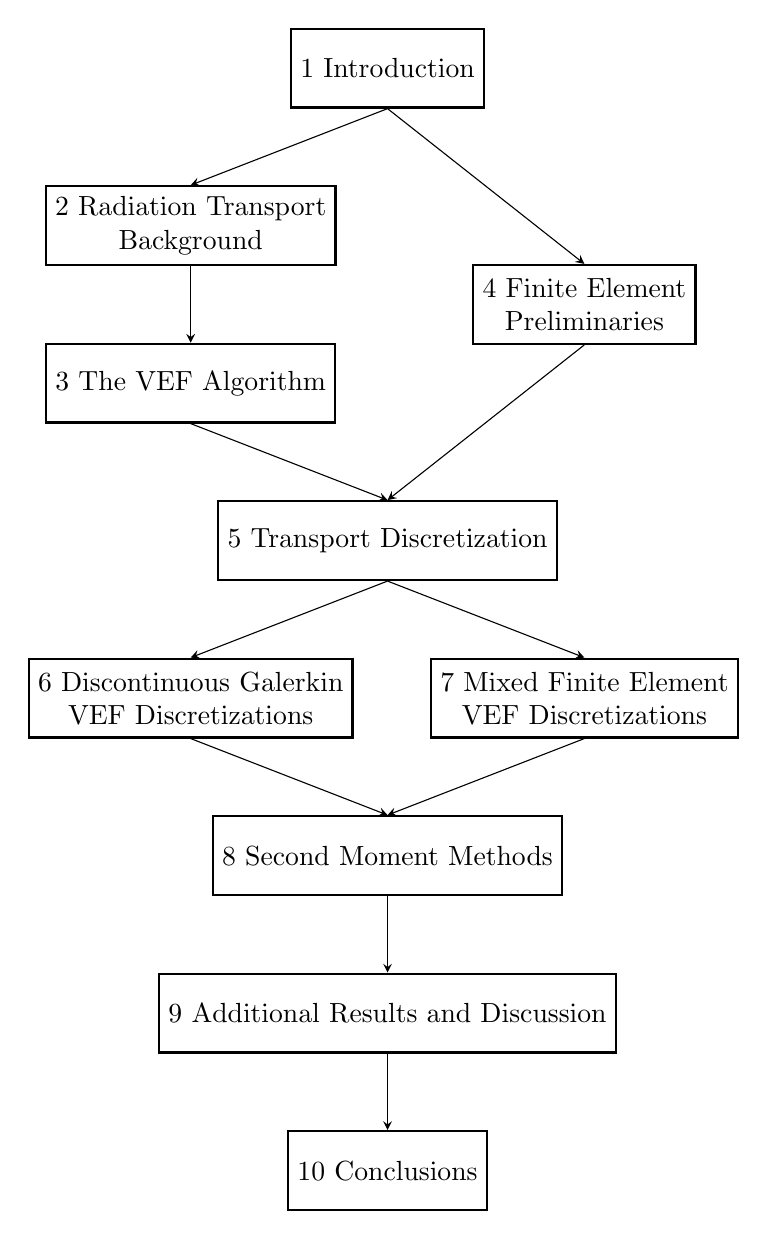
\begin{tikzpicture}[>=stealth]
	\node[node] (intro) {1 Introduction}; 
	\node[node] at ([yshift=-2cm, xshift=-2.5cm]intro) (trans_back) {2 Radiation Transport\\Background};
	\node[node] at ([yshift=-2cm]trans_back) (vef) {3 The VEF Algorithm}; 
	\node[node] at ([xshift=2.5cm, yshift=-3cm]intro) (fem) {4 Finite Element\\Preliminaries}; 
	\node[node] at ([yshift=-6cm]intro) (sn) {5 Transport Discretization}; 
	\node[node] at ([yshift=-2cm, xshift=-2.5cm]sn) (dg) {6 Discontinuous Galerkin\\VEF Discretizations}; 
	\node[node] at ([yshift=-2cm, xshift=2.5cm]sn) (mfem) {7 Mixed Finite Element\\VEF Discretizations}; 
	\node[node] at ([yshift=-4cm]sn) (smm) {8 Second Moment Methods}; 
	\node[node] at ([yshift=-2cm]smm) (disc) {9 Additional Results and Discussion}; 
	\node[node] at ([yshift=-2cm]disc) (conc) {10 Conclusions}; 

	\foreach \a\b in {intro/trans_back, trans_back/vef, intro/fem, 
		vef/sn, fem/sn, sn/dg, sn/mfem, dg/smm, mfem/smm, smm/disc, disc/conc}{
		\draw[->] (\a.south) -- (\b.north); 
	}
\end{tikzpicture}
\end{document}